% Compile with XeLaTeX. This paper specifies a design, not measured results.
\documentclass[11pt,a4paper]{article}
\usepackage[margin=27mm,top=25mm,bottom=26mm]{geometry}
\usepackage{fontspec}
\setmainfont{TeX Gyre Pagella}
\setmonofont[Scale=0.85]{DejaVu Sans Mono}
\usepackage{amsmath,amsthm}
\usepackage{unicode-math}
\setmathfont{TeX Gyre Pagella Math}
\usepackage{microtype,enumitem,tikz}
\usetikzlibrary{arrows.meta,positioning}
\usepackage[hidelinks,bookmarksnumbered=true]{hyperref}
\hypersetup{pdftitle={The ATHENA Hodarium},pdfauthor={ATHENA},
  pdfsubject={A labelled path model and a design for personal multi-device synchronization},
  pdflang={en}}
\urlstyle{same}
\setlength{\parindent}{1.2em}
\setlength{\parskip}{0pt}
\setlength{\emergencystretch}{1.5em}
\linespread{1.04}
\setlist[enumerate]{label=(\roman*),leftmargin=2em,itemsep=4pt,topsep=5pt,parsep=0pt}
\theoremstyle{definition}
\newtheorem{definition}{Definition}[section]
\theoremstyle{plain}
\newtheorem{proposition}[definition]{Proposition}
\newcommand{\Path}{\operatorname{Path}}
\newcommand{\Hom}{\operatorname{Hom}}
\newcommand{\rev}{\operatorname{rev}}
\newcommand{\PP}{\mathcal P}
\newcommand{\HH}{\mathcal H}
\newcommand{\WW}{\mathcal W}
\title{\normalfont\LARGE The ATHENA Hodarium}
\author{}
\date{October 7, 2026}

\begin{document}
\maketitle

\begin{abstract}
We define a hodarium as a finitely generated path category equipped with
path reversal, a word-valued dagger functor, and an existence axiom for
relay-mediated connections. The model distinguishes the existence of a
communication route from the identity and cost of a particular path.
We use it to specify a synchronization system for one person's ATHENA
instances. A central authority manages membership and records conflict
resolutions, while devices exchange saved revisions over automatically
selected, end-to-end encrypted peer-to-peer or relayed connections.
The design separates membership epochs, content revisions, and transport
state; preserves unsaved local work; and requires durable local history
before applying destructive remote changes. We describe admission and
recovery, bounded offline verification, logical database replication,
manual structural merging, and integration with the editor's ownership
model. The resulting specification concerns both mathematical structure
and system behavior; it does not report an implementation or performance
evaluation.
\end{abstract}

\section{Introduction}
\label{sec:introduction}

ATHENA is a structured-document and knowledge-work application. A user
may maintain a substantial collection of documents, attachments,
namespace relations, and derived indexing results on a workstation,
while using a tablet to continue the same work elsewhere. Synchronizing
such a collection involves more than copying changed files. Documents
carry persistent node identities and typed metadata; references depend
on those identities; databases contain both authoritative records and
reconstructible indexes; and an open editor may hold changes that have
not yet been saved. A synchronization mechanism must respect these
distinctions if continuity between devices is to preserve the meaning
of the collection.

The ATHENA Hodarium is designed for this setting. Its members are a
single person's devices, rather than distinct users with separately
negotiated editing rights. Each device retains local storage and can
continue editing without a network connection. A \emph{Vault} is the unit
of participation: a device selects entire Vaults and maps each selected
Vault to a local directory. Membership belongs to the device at the
Hodarium level; selecting a Vault determines the data to replicate, not
a second administrator identity. Replicas of the same Vault are
identified by a stable logical identifier rather than a display name
or an absolute filesystem path.

The system has a centralized control service and decentralized content
storage. One logical \emph{Hodarium Server} administers membership,
publishes authenticated control state, assists discovery, and records
the user's decisions about conflicts. A \emph{Hodarium Relay} is a
separate service that forwards encrypted traffic when devices cannot
communicate directly. Several self-hosted relays may be available,
including relays on a private network and on the public Internet. The
Server and Relay are independent executables with independent deployment
and upgrade lifecycles. Neither service retains Vault contents as a
long-term store. A transfer therefore requires an online sender and an
online receiver, although the receiver may subsequently supply the same
revision to another device after the original sender has disconnected.

Two different kinds of order arise. A communication path orders the
connections through which information passes; a revision history orders
the saved states from which later states derive. The former does not
establish the latter. A fast path carries neither stronger membership
credentials nor a more authoritative document version. Likewise, a
relay's ability to connect two devices says nothing about their current
agreement on a document. The mathematical structure developed below
describes paths and their labels. Membership, revision causality, and
durable application are specified separately and connected through
explicit interfaces.

The first implementation targets Linux and iPadOS. It publishes
successfully saved revisions, including saves performed by ATHENA's
realtime-save mode, and resolves genuine concurrent branches by user
decision rather than automatic selection of a winner. Existing
structural comparison and document-history facilities provide the basis
for merging and recovery. A faulty device may propagate deletions, but
another device must preserve a recoverable preimage before applying
them. This safety requirement is part of synchronization itself, rather
than a request that the user manually create a backup before each
transfer.

\section{Mathematical structure}
\label{sec:mathematics}

We use the convention that $g\circ f$ means first $f$, then $g$.
Sequences of edges and words of labels, in contrast, are written in
the order in which they are traversed. We begin with the categorical
structures needed for the definition. The dagger terminology is
standard; a concrete free construction is described, for example,
in the DisCoPy documentation~\cite{dagger}.

\begin{definition}[Dagger category]
A \emph{dagger category} is a category $\mathcal C$ equipped with an
identity-on-objects functor
$(-)^\dagger:\mathcal C^{\mathrm{op}}\to\mathcal C$ such that, for every
$f:A\to B$,
\[
 f^\dagger:B\to A,\qquad (f^\dagger)^\dagger=f.
\]
In particular, it satisfies
\[
 1_A^\dagger=1_A,
 \qquad (g\circ f)^\dagger=f^\dagger\circ g^\dagger
\]
for every composable pair $f,g$.
\end{definition}

\begin{definition}[Dagger functor]
If $\mathcal C$ and $\mathcal D$ are dagger categories, a
\emph{dagger functor} $F:\mathcal C\to\mathcal D$ is a functor satisfying
\[
 F(f^\dagger)=F(f)^\dagger
\]
for every morphism $f$ of $\mathcal C$.
\end{definition}

A quiver $Q=(V,E,s,t)$ consists of vertices $V$, edges $E$, and source
and target maps $s,t:E\to V$. Loops and parallel edges are permitted.
Its free path category $\Path(Q)$ has objects $V$ and morphisms the
finite composable sequences of edges. The empty path at $A$ is $1_A$,
and composition is concatenation. Consequently, every morphism has a
unique edge-sequence representation; there are no equations between
distinct sequences. This is the usual path-category
construction~\cite{pathcat}. A finite quiver need not have a finite
path category, since cycles can be traversed arbitrarily many times.

We also need a target for the labels of paths. For an alphabet $\Sigma$,
let $\Sigma^*$ be the free monoid of finite words, with empty word
$\epsilon$. Define a one-object category $\WW_\Sigma$ by
\[
 \operatorname{Ob}(\WW_\Sigma)=\{*\},\qquad
 \operatorname{End}_{\WW_\Sigma}(*)=\Sigma^*,\qquad
 v\circ u:=uv.
\]
The identity is $1_*=\epsilon$. The composition convention makes first
traversing $u$ and then traversing $v$ produce the word $uv$.
Equip $\WW_\Sigma$ with the dagger
$u^\dagger=\rev(u)$, where $\rev$ reverses a word and fixes each letter.
Indeed, $\rev(uv)=\rev(v)\rev(u)$, so this is a contravariant involution
for the stated composition convention.

The complete structure can now be given in a single definition.

\begin{definition}[Hodarium]
\label{def:hodarium}
A \emph{hodarium} is a tuple
\[
 \HH=(Q,R,p,\dagger,C)
\]
with the following data and requirements.
\begin{enumerate}
\item $Q=(V,E,s,t)$ is a finite quiver, $R$ is a finite set of relay
labels, and $p\notin R$ is the distinguished peer-to-peer label.
Write $\Sigma=\{p\}\sqcup R$ and $\PP=\Path(Q)$.

\item The \emph{dagger axiom} requires a specified involution on
generating edges, $e\mapsto e^\dagger$, satisfying
\[
 s(e^\dagger)=t(e),\qquad t(e^\dagger)=s(e),\qquad
 (e^\dagger)^\dagger=e.
\]
The dagger on $\PP$ is its extension by path reversal:
\[
 (e_1,\ldots,e_n)^\dagger=(e_n^\dagger,\ldots,e_1^\dagger),
 \qquad 1_A^\dagger=1_A.
\]

\item The \emph{color functor} $C:\PP\to\WW_\Sigma$ is a dagger
functor sending each generating edge to a one-letter word. Its
restriction is denoted $c_0:E\to\Sigma$. Thus
\[
 c_0(e^\dagger)=c_0(e),\qquad
 C(e_1,\ldots,e_n)=c_0(e_1)\cdots c_0(e_n).
\]

\item The \emph{relay axiom} requires that, for every $r\in R$, every
pair of generating edges $a:A\to X$ and $b:Y\to B$ with
$c_0(a)=c_0(b)=r$, and every path $T\in\Hom_{\PP}(X,Y)$, there is
a generating edge $h:A\to B$ with $c_0(h)=r$.
\end{enumerate}
The category $\PP$ is the communication category of $\HH$.
\end{definition}

The data in this definition are compatible without imposing additional
relations on paths. Given an edge-reversing involution and a labelling
$c_0$ that is constant on its orbits, freeness gives exactly one functor
$C$ with that restriction. Reversing a path reverses the order of its
labels and leaves the individual labels unchanged, proving that this
functor preserves daggers. The relay axiom then restricts which labelled
generating graphs are admissible. It is a condition on the existence of
edges, rather than a quotient of the path category.

In the network interpretation, vertices are ATHENA instances and
generating edges are available single-step device-to-device connections.
An edge $A\xrightarrow{r}B$ denotes the physical communication
$A\to r\to B$ through the relay labelled $r$; the relay itself is not
a vertex. An edge labelled $p$ denotes a direct connection. Parallel
edges may record distinct connections between the same devices. The
model is taken at a fixed network state and within a fixed domain of
eligible communication. It describes connections that can be
established, not merely sessions that happen to be open.

The relay axiom says that if a path starts and ends with connections
through the same relay, then its endpoints also admit a single
connection through that relay. The middle path may be empty, monochromatic,
or mixed. Figure~\ref{fig:relay} illustrates the assertion. It does not
assert $h=b\circ T\circ a$: the one-edge route and the longer route
remain different morphisms and can have different costs. In particular,
the axiom does not invent an intermediate device through which two
unrelated relays could be connected.

\begin{figure}[htbp]
\centering
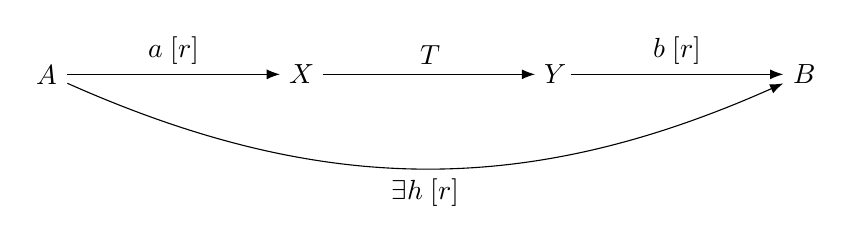
\begin{tikzpicture}[>=Latex,node distance=27mm]
\node (a) {$A$}; \node[right=of a] (x) {$X$};
\node[right=of x] (y) {$Y$}; \node[right=of y] (b) {$B$};
\draw[->] (a)--node[above]{$a\;[r]$}(x);
\draw[->] (x)--node[above]{$T$}(y);
\draw[->] (y)--node[above]{$b\;[r]$}(b);
\draw[->] (a) to[bend right=24] node[below]{$\exists h\;[r]$}(b);
\end{tikzpicture}
\caption{The relay axiom supplies a generating edge with the same
endpoints. The two displayed paths are not identified.}
\label{fig:relay}
\end{figure}

\begin{proposition}[Monochromatic completeness]
\label{prop:complete}
For $r\in R$, let $Q_r$ retain all vertices of $Q$ and precisely its
$r$-labelled generating edges. Every connected component of the
underlying undirected graph of $Q_r$ has an $r$-labelled edge in each
direction between any two distinct vertices. Every vertex incident
with an $r$-labelled edge also has an $r$-labelled loop.
\end{proposition}
\begin{proof}
Use the specified dagger to orient a connecting chain in the desired
direction. A chain of length one is already the required edge. For a
longer chain, use its first and last edges as $a,b$ and the intervening
path as $T$ in the relay axiom. For a vertex incident with an
$r$-labelled edge, orient that edge to start there and apply the axiom
to it and its dagger, with the empty middle path. This supplies the loop.
\end{proof}

Isolated vertices require no such loop. Completeness allows parallel
edges and does not impose uniqueness of a connection. Moreover, the
full relay axiom is stronger than closure under purely $r$-labelled
chains: it also applies when the intervening path uses other labels.
This matters when identifying the communication domain of a deployed
relay. Pair-specific restrictions cannot be silently hidden behind a
label for which the axiom is assumed. Conversely, a partial observation
of the network need not itself display all the edges whose existence
the model permits.

The color functor assigns a well-defined word to every path and satisfies
\begin{equation}
 C(g\circ f)=C(f)C(g),\qquad C(1_A)=\epsilon,
 \qquad C(f^\dagger)=\rev(C(f)).
 \label{eq:color}
\end{equation}
Define the length of a path by $\ell(f)=|C(f)|$. Then length is additive
under composition and invariant under the dagger. A nonempty path is
\emph{monochromatic} when its word contains only one distinct letter;
otherwise it has mixed color. The empty word is reserved for identities.
For example, a path with labels $r,p,s$ has word $rps$, and its reversal
has word $spr$. Different paths can have the same color word, because
the functor forgets device and connection identities.

These distinctions have immediate operational consequences. The words
$p$, $pp$, and $\epsilon$ are distinct: two successive direct connections
do not imply a direct connection between the outer devices. Similarly,
$r$ and $rr$ remain distinct even when the relay axiom supplies a
shortcut. A nonempty round trip $f^\dagger\circ f$ has length
$2\ell(f)$ and is not the empty path. Length counts device-to-device
steps, not physical IP hops; a relay-mediated connection is one such
step. Nothing in the dagger axiom requires equal throughput or latency
in opposite directions.

The path category is not a scheduler. A practical implementation
maintains a bounded set of candidate connections and their measured
costs, rather than enumerating all possible walks.
Changing connectivity or eligibility changes the generating graph.
Likewise, propagation in which $A$ supplies $B$ and, later, $B$ supplies
$C$ is a sequence across time; it does not require both connections to
exist in the same snapshot. The revision model in
Section~\ref{sec:replication} provides the persistent identities needed
to describe that propagation without confusing it with a new edit.

\section{Membership, authority, and trust}
\label{sec:membership}

The Hodarium Server is the single logical authority for membership.
It serializes admission and expulsion and publishes a signed state
binding the Hodarium identifier, protocol version, monotone membership
revision, fresh random epoch identifier, and the corresponding member
set or an authenticated commitment to it. Random identifiers are not
reused within the Hodarium. The revision establishes order, whereas
the epoch identifier provides an equality token for the current
membership state. Clients persist the highest accepted control state
and verify that its fields and membership data belong to the same
signed publication.

The authority is trusted to administer membership, but it is not a
document repository. It holds its own signing identity and the public
identities of members, not their private keys or document-decryption
keys. Compromise of this authority can admit an adversary to whom an
honest device may subsequently send data; end-to-end encryption does
not remove that administrative trust. A relay occupies a different
position. It may observe traffic timing, endpoints, and volume, or
refuse service, but it is not trusted with plaintext or membership
decisions. A compromised member can read its local plaintext, and
expulsion cannot recover copies it already possesses.

Administration takes place in a Web panel authenticated with passkeys
through WebAuthn~\cite{webauthn}. Administrative browser sessions and
synchronization device identities are separate. The user can therefore
admit a new device from an authenticated browser without requiring an
older ATHENA instance to be online. Admission, expulsion, authenticator
changes, and recovery configuration require recent user verification.
The implementation uses a maintained WebAuthn library and validates
the challenge, relying-party identity, origin, and verification result,
alongside ordinary session expiry and cross-site request protection.
Several authenticators can be registered so that loss of one does not
make routine administration impossible.

A joining device first authenticates the configured HTTPS service,
generates a long-lived local key, and submits its public key with proof
of possession. The Server creates a pending request with a high-entropy
private retrieval credential and a short numeric code for the user.
The displayed code rotates on a timescale of tens of seconds; thirty
seconds is an initial operational choice, while code length and attempt
budgets remain parameters of the implementation. The user enters the
code into the authenticated panel, examines the pending request, and
approves it. Approval binds the exact request, device public key, and
Hodarium. The device then proves possession again and retrieves its
admission using the private request credential.

The short code locates a request; it is neither an administrator
password nor a bearer credential for membership. Requests expire,
approval is consumed once, and code rotation does not reset the
request's aggregate failure budget. Rate limits are enforced by the
service, rather than assumed from correct client behavior. Device
names are explanatory labels, not evidence of identity. This division
between a device request and approval in a separate browser resembles
the device authorization pattern~\cite{deviceflow}; the rotating display
code and proof-of-possession bindings are explicit requirements of
this design, not claims about that RFC's exact protocol.

Each admitted device keeps its own long-lived private identity in the
platform's protected storage. Linux integration uses a maintained
client of a system secret store such as Secret Service~\cite{secretservice};
iPadOS uses Keychain~\cite{keychain}. A locked or unavailable store
suspends operations requiring the key and produces an actionable
status. It does not cause silent fallback to a plaintext key file.
This avoids routine copying of key files or repeated synchronization
password entry, without claiming protection against complete compromise
of the local operating system.

Initial administration is established through a server-local bootstrap
operation that creates a one-time high-entropy credential for enrolling
the first passkey and a recovery public key. An anonymous first visitor
cannot claim the service. The corresponding recovery private key is
kept offline by the user. Recovery can restore administrative access,
invalidate old sessions, register new authenticators, and establish a
new trusted control state. Re-admitting a device creates a new member
instance rather than reviving old sessions. Administrative recovery is
independent of the existence of any current member, so expelling the
last device does not destroy the ability to admit another. It also does
not reconstruct lost document contents.

An authenticated data session is admissible only when both devices
verify possession of the declared member keys, agree on the Hodarium
and epoch, find the peer's member instance in that state, and retain
valid evidence of a sufficiently recent check with the Server. The
epoch identifier itself is not secret and conveys no authority in
isolation. On a mismatch, peers exchange a protocol-level refresh
request; they do not ask the user to settle the mismatch in a dialog.
Each contacts its configured authority rather than following an
untrusted replacement address supplied by the other peer.

Offline verification is bounded by twenty-four hours after the last
fresh authenticated validation with the Server. A previously signed
member list obtained from another device cannot renew this period.
Even if membership has not changed, renewing freshness requires a
current exchange with the authority. The client tracks membership
version and freshness separately, so replaying an old state cannot
simulate a new online check. System-clock changes, restart, or suspension
must not extend the bound indefinitely; uncertainty about the remaining
period requires revalidation. Existing sessions are subject to the same
expiry and membership checks as new ones.

This rule deliberately admits a bounded propagation delay for
expulsion. Two disconnected devices with the same still-valid old
epoch can continue exchanging data until they learn the new state or
their offline period expires. After expiry, synchronization pauses,
but local reading, editing, and saving remain available. Receiving an
expulsion never erases the expelled device's existing files. Ordinary
saves and conflict decisions do not advance the membership epoch,
because document causality and authority freshness are different
state variables.

Control recovery must also address rollback. Restoring an old Server
database cannot simply reactivate an older member set. Recovery needs
an explicit new recovery generation, trusted re-establishment of the
authority state where necessary, and client-side rollback checks.
Control signatures authenticate the authority's statements; they do
not, by themselves, prove that a compromised authority has not issued
inconsistent statements. The design therefore makes its trust in the
single administrative authority explicit rather than attributing
stronger guarantees to the epoch mechanism.

\section{Communication and route selection}
\label{sec:communication}

Devices publish reachability and rendezvous information through the
Server for access by eligible members. The user configures which
self-hosted relays may be used and any traffic or energy restrictions.
The client determines the active connection automatically. Its initial
candidate set consists of direct connections and connections through
one allowed relay; the first implementation does not forward traffic
between relay services. Both endpoints of a relayed session must
eventually reach the same relay, even if they initially registered
with different services. No usable path is a distinct state from
failed authentication or temporarily unavailable content.

A relay uses short-lived, difficult-to-guess rendezvous handles rather
than publicly enumerable Vault paths. It has its own service identity,
resource-access credentials, connection and traffic limits, bounded
buffers, and idle timeouts. Such credentials authorize use of the
relay's resources, not admission to a Hodarium. The service can support
several Hodariums without becoming a member of any of them. It holds
neither device-identity secrets nor recovery credentials nor document
keys. Independent relay access control is nevertheless necessary to
avoid turning a public deployment into an unrestricted traffic service.

The devices establish an authenticated end-to-end encrypted session
using a mature transport implementation. When a relay is involved,
this session remains inside the relayed connection: decrypting at the
relay and then encrypting a second outgoing connection would violate
the boundary. The peer identity is bound to the device key, member
instance, Hodarium, and current epoch, with freshness tied to the
current handshake. Existing relaying designs provide precedents for
separating relay access from peer authentication~\cite{relay}. The
particular cryptographic suite and wire representation are implementation
choices subject to review; the design does not require inventing a
new encryption protocol or maintaining a single shared plaintext
master key on every member.

The authority needs only the control metadata required for membership,
discovery, and decisions. Filenames, Vault-relative paths, document
contents, and guessable plaintext digests should not be exposed there
by default. If a content identifier or commitment could disclose
low-entropy information, its representation needs an independently
reviewed confidentiality mechanism. End-to-end protection does not
conceal all traffic analysis: relays still observe connection and
volume information, and the authority observes membership and the
control operations submitted to it.

Transfer requests refer to immutable revisions and verifiable chunks.
Received bytes enter staging storage; validation and the local apply
protocol precede any replacement of the current object. Acknowledgements
distinguish receipt of bytes, durable storage of a replica, and
application as the current revision. Resumption after failure cannot
equate these stages. Changing a route preserves the transfer and revision
identities, resumes at a verified boundary, and performs the required
freshness checks without applying already acknowledged data twice.

Route selection is based on measurements of the complete device-to-device
connection. The client records setup cost, round-trip time, useful
throughput, failure rate, and stability. Samples are associated with
the peer, particular candidate connection, direction, local network
context, and an expiry time. The completeness of a relay component in
Proposition~\ref{prop:complete} identifies possible connections, not
their performance. A ping from one device to the relay is not a
measurement of the entire path to another device, and a reverse
connection need not have the same cost as its dagger mate.

The relevant objective depends on the transfer. Small control exchanges
are sensitive to setup and latency, whereas a large attachment is
usually more sensitive to throughput. One initial estimate of completion
time for a candidate $\pi$ is
\begin{equation}
 \widehat T_\pi(S)=\widehat T_{\mathrm{setup},\pi}
       +k\,\widehat{\mathrm{RTT}}_\pi+\frac{S}{\widehat B_\pi},
 \label{eq:cost}
\end{equation}
where $S$ is the useful payload size, $k$ estimates the protocol's
remaining round trips, and $\widehat B_\pi$ is measured throughput in
the relevant direction. Failure and stability policies supplement this
estimate. Equation~\eqref{eq:cost} describes a scheduling heuristic,
not an algebraic property of color words. In particular, the implementation
does not assume that a direct connection must outperform a relay.

Measurement consumes resources and can distort its own observations.
Connection probes have bounded concurrency; throughput probes are
scheduled so that simultaneous tests do not simply saturate a shared
uplink. Recent valid samples provide an initial choice, actual transfers
update those samples, and active tests are bounded when observations
are insufficient. Network changes, wake-up, failure, and expiry trigger
re-evaluation. Idle clients do not run continuous full-bandwidth tests
or measure every pair of vertices merely because a relay component is
complete. Battery state, metered connectivity, and operating-system
suspension constrain probing, but do not change revision semantics.

A healthier or faster candidate replaces a working connection only
after a sustained advantage, using hysteresis and a minimum holding
period to avoid oscillation. Failure permits immediate fallback.
The two endpoints coordinate the route selected for a transfer instead
of independently switching in conflicting directions. The first
implementation uses one active data route per transfer with failover,
rather than requiring concurrent striping across all available routes.
The interface reports the active path, measured rate, and reasons for
waiting or switching; it does not require the user to choose a preferred
relay for each exchange.

The storage assumptions remain independent of these transport choices.
A relay has only transient forwarding buffers, and the Server is not
an offline content mailbox. If $A$ sends a revision to $B$, then $B$
can supply it to $C$ after $A$ disconnects, preserving its identity and
ancestry. If every holder of the content is offline, control records
can describe the revision but cannot deliver it. A claim of an additional
durable replica therefore requires acknowledgement from another device.
Separate one-way backup to a service such as Nextcloud remains useful;
each device uses an isolated backup destination so that independent
backup jobs do not overwrite one another or become an accidental
synchronization mechanism.

\section{Replication and conflict resolution}
\label{sec:replication}

A Vault contains several kinds of state with different replication
rules. Source documents, compound virtual document definitions, images,
PDFs, attachments, and user-maintained styles or sorters are persistent
source objects. Namespace membership and ordering, Materials metadata,
manual artifact corrections, and rejected-name records are authoritative
logical records. Artifact extractions, model judgments, and embeddings
are derived results that may be reused when their complete input
contracts match. Location indexes, scan state, task queues, locks, and
temporary files are local operational data. Device credentials, local
directory mappings, and device-specific backup preferences are private
configuration rather than remote replacement targets.

These distinctions follow semantics, not filenames. Copying a live
SQLite or LMDB database, its journal, or an entire internal directory
does not implement replication of its logical entities. Authoritative
records are exchanged with stable identities, revisions, relationships,
and tombstones. Independent entities can advance independently, while
related changes require explicit batch or recovery boundaries. Source
node UUIDs and the persistent bindings that preserve artifact identities
travel with authoritative data; receiving devices rebuild their local
location indexes. The storage format of a particular cache is not an
additional source of reference identity.

Reusable results are checked against source identity, extraction role,
model version, and the actual model-input fingerprint. Matching results
can be installed without recomputation, while stale results remain
distinguishable from current ones. A derived result cannot overwrite a
manual decision, alter source content, or cause a new revision merely
because an index was refreshed. A compound virtual document replicates
its definition and relevant namespace relations; reuse of its macro
computation cache requires the corresponding dependency fingerprint.
Downloaded styles and sorter programs remain subject to local execution
policy. Receiving a file does not grant it execution privileges.

Each synchronization object has a stable identity, and each saved
revision has an immutable identifier, a finite parent set, an integrity
binding to its content or deletion state, and the necessary format and
semantic versions. The parent relation forms an acyclic revision graph.
Write $u\preceq v$ if $u=v$ or $u$ is an ancestor of $v$. This relation,
rather than a device clock or file modification time, determines whether
one state succeeds another. Origin-device information is retained for
audit but does not turn each device into a separate user authority.

Receiving an already known revision is idempotent. A descendant of the
current revision can advance it once local application conditions are
satisfied; an ancestor does not roll it back. Incomparable revisions
are retained as branches. Deletion is represented by a tombstone
revision, and rename is attached to the stable object identity, so
deletion concurrent with editing or renaming remains expressible.
Identical visible text does not erase distinct causal histories, nor
does it justify ignoring changes to node identities, properties,
references, or attachments. Garbage collection of historical payloads
must preserve the ancestry information still needed for correct
comparison and duplicate suppression.

Publication occurs only after a successful save. In realtime-save mode,
each successful local save makes a revision eligible for synchronization;
in ordinary mode, unsaved edits remain local. Queued work may be coalesced
without losing branch relationships, but neither a failed save nor a
partially written file may be announced as a published revision. The
same boundary applies when the application closes: content that the
user discards without saving is not published as an incidental consequence
of shutdown. Loss of connectivity affects delivery, not the ability to
save locally.

A remote successor arriving while a document has unsaved edits is
stored as a remote candidate. It does not force a save or overwrite the
open buffer. The user may save a local branch, explicitly discard the
draft before applying the remote state, or enter a merge workflow.
Even an apparently clean open buffer is updated through its owning
BufferActor, which rechecks the expected revision at the point of
application. This prevents an edit made while a background operation
was waiting from being overwritten by an earlier decision that the
buffer was clean.

Conflicts are resolved by the user through ATHENA's structural comparison
facilities. The interface presents a usable common ancestor when one
is available, the competing branches, and an editable result. Comparison
includes atomic and compound node identities, typed properties,
structured names, reference collections, and content. XML line differences
are not an adequate substitute. Existing two-tree comparison can supply
difference ranges, but three-way interaction and metadata-aware
presentation require an explicit merge layer. When the common ancestor's
payload is unavailable, the interface states that limitation rather
than inventing a three-way base.

The user can adopt one branch, select and edit portions of several
branches, or deliberately preserve separate objects. Merging preserves
the identity of a logical object; duplication as a new object generates
new identities and remaps internal references according to ATHENA's
copy semantics. Metadata conflicts, delete--modify conflicts, and
path collisions need their own intelligible representations. In every
case, a resolution revision records all the branches it resolves as
parents. If $X$ and $Y$ are the conflicting heads and $M$ adopts the
content of $X$ unchanged, it still records
\[
 \operatorname{parents}(M)=\{X,Y\}.
\]
The relation to $Y$ expresses that it was considered and resolved;
without it, another device could repeatedly rediscover the same conflict.

The Server makes that decision authoritative for its stated scope
without inspecting the merged content. After durably storing the result,
the client submits a signed request binding the Hodarium, Vault, object,
conflict identifier, exact branch set, expected decision version, and
result identifier. The authority checks current membership and
conditionally commits the decision. Competing stale submissions cannot
each become the accepted decision for the same conflict version.
A client whose submission loses the race retains its local merge result
and learns the already committed decision; user work is not discarded
as a side effect of control-plane concurrency.

Acceptance of a decision and acquisition of its result are separate
events. Other devices retrieve the result from any online member that
holds it and validate its identity, parent set, format, and content
before applying it. A device that knows the decision but lacks the
payload remains in a waiting-for-content state; it cannot appoint a
different winner because the submitting device disconnected. When the
Server is unavailable, the user can prepare a merge draft but cannot
claim a globally committed decision. If a previously unknown offline
branch later arrives and is not already accounted for by the accepted
history, it is compared causally and may create a new conflict. An old
decision does not dispose of unseen concurrent work.

Control records are recovered through persistent cursors, with push
notifications used only to reduce latency. A conflict suspends the
affected objects rather than the entire Vault. Successful resolutions,
new descendants, and restored revisions propagate through the same
identity-preserving data mechanism. Conditional on eventual delivery
and the user's resolution of remaining branches, participating replicas
can converge on the same accepted states; the design does not assert
instantaneous equality during disconnection or unfinished conflict
handling.

\section{Durable application and native integration}
\label{sec:integration}

Remote changes become local state only through an application procedure
that preserves recovery information. Before replacing or deleting an
object, the receiving device durably records its previous state in
protected File History. The rule applies to ordinary updates and to
large batches of remote deletions, without relying on an additional
confirmation dialog for a sufficiently large batch. Disk exhaustion,
permission failure, or failure to capture history suspends the affected
application. The system cannot first destroy the current object and
then attempt to make the operation recoverable.

An apply operation begins by validating the staged revision and its
content and checking the expected local state. It obtains a consistent
preimage, commits that preimage to history, and persists an application
intent describing the expected old revision and the staged replacement.
At the commit boundary it checks the precondition again, applies the
replacement, and records the applied revision before acknowledging
completion. If the precondition has changed, the operation is reconsidered
rather than overwriting the newer state. Following a crash, the intent
log identifies incomplete operations for idempotent completion or rollback.

The filesystem and several logical databases do not share an implicit
transaction. Per-object commit boundaries and cross-object recovery
records must therefore be explicit. A rename coupled to namespace
changes, for example, needs enough information to restore or complete
the associated relationships. A batch deletion requires a manifest
from which the batch can be restored without asking the user to recall
every former filename. Historical capture includes attachments and
authoritative logical records as well as document bodies; protecting
only the \texttt{.ath} payload does not establish recoverability of a
Vault.

ATHENA's existing history storage, reconstruction, and restoration
interfaces can be reused, with capture reasons for synchronization
replacement, deletion, and conflict application. Ordinary asynchronous
submission to a history queue is not sufficient for the pre-application
barrier: the apply coordinator needs an explicit durable-success result.
Restoring a historical version creates a new revision derived from
the appropriate current history, rather than turning back a revision
clock or reviving old membership credentials.

Protected history, application journals, and device credentials lie
outside ordinary remote file replacement. A remote tombstone or changed
Vault preference cannot delete them or shorten a device's protection
period. Retention and space-management policy must not silently remove
the only recovery copy while treating a destructive operation as safely
protected. The precise retention parameters need an explicit operational
policy, but their source of authority is local. Independent backup
remains necessary for losses outside this boundary, including complete
device compromise or simultaneous loss of all replicas and their
histories. A recovery key restores administrative control, not absent
payloads.

Within the client, ownership follows the existing editor architecture.
Live document trees are read and modified by their owning BufferActor;
background work uses detached snapshots or immutable byte representations.
The network submits version-conditional application requests rather
than manipulating editor state. Tree modifications preserve UUIDs,
typed properties, observer notifications, and undo semantics. Conversion
through an intermediate representation that discards metadata is not
an acceptable way to apply a remote edit.

The implementation separates control-state handling, transport scheduling,
revision bookkeeping, Vault-specific record adaptation, history-backed
application, and merge interaction. These responsibilities need not be
separate processes; the independent Server and Relay executables are
the required process boundaries. Fixed worker pools, bounded queues,
and backpressure prevent the number of files or candidate routes from
creating unbounded concurrency. The GUI does not wait synchronously
for membership refresh, a network operation, or a Vault scan. Native
internal interfaces connect synchronization to the editor; external
plugin request machinery does not become an additional dependency of
document application or rendering.

Change discovery primarily follows successful-save notifications and
filesystem observations, supplemented by infrequent reconciliation.
Unchanged stat fingerprints allow reuse of verified scan results;
known changes, invalidation, and integrity checks determine when content
must be reread. External editing, atomic replacement, and renaming
are reconciled against object state rather than event order alone.
Synchronization application and index rebuilding retain their origin
so that local maintenance writes do not return as fresh user edits.
Idle operation should not repeatedly parse the entire Vault or rewrite
database pages merely to maintain polling state.

Platform adaptation preserves the same data semantics. iPadOS may
suspend the application and interrupt connections; resumption rechecks
membership freshness, staged transfer state, and available routes before
continuing. Linux and iPadOS use their respective protected key storage
and network lifecycle interfaces. Protocol paths are Vault-relative,
and receiving devices reject traversal, unsafe links, and filename
collisions caused by case or normalization rules. Attachments retain
stable synchronization identities through renames. Format versions,
UTF-8 validity, node metadata, and resource budgets are checked before
content becomes active.

The administrative interface is a conventional Web application served
by the Hodarium Server. It uses maintained framework, form, component,
and WebAuthn implementations, rather than a bespoke collection of
hand-written controls. Its shared theme uses square corners
(\texttt{border-radius: 0}), consistent with ATHENA, and supports keyboard,
touch, and assistive navigation. The principal views expose membership,
pending requests, reachability, synchronization summaries, conflict
decisions, authenticators, recovery configuration, and audit records.
Document merging remains in the native client; the panel receives no
document-decryption keys. A production deployment serves built assets
without requiring a permanently running frontend development server.

Optional notifications use a replaceable mail integration, such as a
Resend-compatible service or SMTP. They report membership and security
events but do not authorize them. Messages lead to the authenticated
panel and exclude approval credentials, short verification codes,
recovery secrets, document paths, and contents. A persistent, deduplicated,
rate-limited queue supports retry without allowing anonymous requests
to generate unlimited mail. A delivery failure cannot reverse an
already committed admission or expulsion, and provider acceptance is
not represented as proof that the user received the message.

Service operation must preserve identity as well as data. Stable HTTPS
origins and relying-party identifiers support continued passkey use.
Server migration and changes to certificates or authority keys require
explicit trusted transition procedures, not disabled verification.
Control backups cover the member log, authority identity, administrator
credentials, recovery public key, and decision log, with the rollback
protections described in Section~\ref{sec:membership}. Relay credentials
and deployment remain independently managed. A relay failure may cause
route switching, whereas authority unavailability invokes the bounded
offline-verification rule; the interface distinguishes these cases.

Operational errors enter ATHENA's normal warning and error channels
and its Error Messages view, with transient notifications serving only
as supplementary presentation. Audit records identify the action,
request, actor, and outcome without recording secrets or Vault plaintext.
Repeated failures may be aggregated with counts, while normal waiting
is not repeatedly reported as an error. Content traffic and measurement
traffic are accounted for separately so that probing costs are visible.
Pausing synchronization for a Vault does not disable local editing or
history.

The remaining realization choices concern maintained libraries,
cryptographic suites, wire encodings, probing thresholds, polling
intervals, and retention parameters. They are reviewed and versioned
without changing the structural and behavioral contracts above.
Acceptance work can be organized around those contracts: reversal and
color preservation; admission bound to possession of the approved key;
freshness that cannot be extended by replay; idempotent transfer across
route changes; preservation of unsaved edits; conditional conflict
decisions; and recoverability of interrupted or destructive application.
Isolated Vaults and representative copies provide the appropriate test
environment before explicit production enrollment. These obligations
connect the mathematical model to a concrete system while keeping
path existence, administrative authority, and document correctness as
distinct questions.

\begin{thebibliography}{9}
\raggedright

\bibitem{dagger}
DisCoPy contributors.
\emph{What is a diagram?} Dagger categories and free constructions.
\url{https://docs.discopy.org/en/interaction-readme/notebooks/diagrams.html}.

\bibitem{pathcat}
Musa Al-hassy.
\emph{Graphs are to categories as lists are to monoids}.
\url{https://alhassy.com/PathCat}.

\bibitem{webauthn}
World Wide Web Consortium.
\emph{Web Authentication: An API for accessing Public Key Credentials,
Level 3}.
\url{https://www.w3.org/TR/webauthn-3/}.

\bibitem{deviceflow}
W. Denniss, J. Bradley, M. Jones, and H. Tschofenig.
\emph{OAuth 2.0 Device Authorization Grant}.
RFC 8628, 2019.
\url{https://www.rfc-editor.org/rfc/rfc8628.html}.

\bibitem{secretservice}
freedesktop.org.
\emph{Secret Service API}.
\url{https://specifications.freedesktop.org/secret-service/latest/}.

\bibitem{keychain}
Apple.
\emph{Keychain services}.
\url{https://developer.apple.com/documentation/security/keychain-services}.

\bibitem{relay}
Syncthing contributors.
\emph{Relaying}.
\url{https://docs.syncthing.net/users/relaying.html}.

\end{thebibliography}
\end{document}
